\chapter{What is established, and what is not}\label{ch:status}

\begin{center}\small
\begin{longtable}{@{}p{0.47\textwidth}p{0.20\textwidth}p{0.22\textwidth}@{}}
\caption{Status of the book's principal claims.}\label{tab:status}\\
\toprule claim & status & where \\\midrule\endfirsthead
\toprule claim & status & where \\\midrule\endhead
\multicolumn{3}{@{}l}{\emph{Physics}}\\
Landauer cost per bit at 37~\textdegree C is $2.97\times10^{-21}$ J & \calc & Ch.~\ref{ch:landauer} \\ \rowrule
$M=\dGATP/R\Tb=20.94$; one ATP pays for 30.2 Landauer bits & \calc & Ch.~\ref{ch:landauer} \\ \rowrule
methylation maintenance is a negligible part of a cell's energy budget & \calc & Ch.~\ref{ch:landauer} \\ \rowrule
$H(\beta)$ is the entropy of the DNA copies at one CpG; two branches & \derived & Ch.~\ref{ch:surface} \\ \rowrule
Smarr: a horizon's $T_HS$ is half its $Mc^2$ & \derived & Ch.~\ref{ch:ledgers} \\ \rowrule
a cell pays half its cost as motion and half as record & \conjecture & Ch.~\ref{ch:ledgers} \\ \rowrule
saturation at the horizon and in the cell share one structure & \analogy & Ch.~\ref{ch:floorbreach} \\ \rowrule
departure from the floor means loss of maintained fidelity, not of energy & \conjecture & Ch.~\ref{ch:floorbreach} \\ \rowrule
\multicolumn{3}{@{}l}{\emph{The gauge}}\\
Met-A $=$ mean $H(\beta)$ on the cell's identity sites over the same cell type's healthy reference & definition & Ch.~\ref{ch:meta} \\ \rowrule
neutrophil reference on EPIC: 6 physical arrays, 6,000 identity sites, floor 0.330263 bits & \calibrated & Ch.~\ref{ch:meta} \\ \rowrule
held-out Met-A of the six reference arrays, SD 0.020 & \measured & Ch.~\ref{ch:meta} \\ \rowrule
Met-A commissioned 2026-10-09 on isolated neutrophils, EPIC v1 & \measured, commissioned & Ch.~\ref{ch:meta} \\ \rowrule
IAM-A $=\varepsilon/\varepsilon_{\rm pred}(L)$, each sample against its own loose share; band v1 $0.779$--$1.055$ & definition; line \measured & Ch.~\ref{ch:iama} \\ \rowrule
$E_{\rm hold}=3.41\,\kB T$, $\varepsilon_0=0.032$, $\varphi=E_{\rm hold}/M=0.163$ & \measured, \calc & Ch.~\ref{ch:iama} \\ \rowrule
neutrophil position $P=1.149$ (3 donors, whole files, 1.140--1.155), earlier position form, now a development flag & \measured & Ch.~\ref{ch:iama} \\ \rowrule
IAM-Atlas v2.1, 79 cells: commissioned 2026-10-16 for three cell references (450K) and the colon and lung blind sites & \measured & Ch.~\ref{ch:atlas} \\ \rowrule
Deconvolution tool (atlas v2.1): commissioned 2026-10-17 for blood-cell shares (neutrophils, monocytes, CD4 T, CD8 T; arrays) & \measured & Ch.~\ref{ch:atlas} \\ \rowrule
IAM-A (sequencing, its own reference): commissioned 2026-10-17 on healthy blood CD8 T cells & \measured & Ch.~\ref{ch:iama} \\ \rowrule

Met-A C-score baseline 1.0103 (blocks of 10); healthy band 0.877--1.152, read one-sided; commissioned on whole blood 2026-10-15 & \calibrated & Ch.~\ref{ch:cscore} \\ \rowrule
$A=1$ healthy in the middle; Normal $=1\pm0.05$ & design tolerance & Ch.~\ref{ch:gauge} \\ \rowrule
floor $\Hmin$: Met-A $1\times10^{-7}$, IAM-A $1$--$2\times10^{-8}$ (the sample's own); surface full: Met-A 3.03, IAM-A $0.5/\varepsilon_{\rm pred}(L)$, 6.68--12.42; C-score far end 45 & \calc & Ch.~\ref{ch:gauge} \\ \rowrule
breach and the cancer region on this gauge & \openprob{} (to be measured) & Ch.~\ref{ch:gauge} \\ \rowrule
the Met-A floor ($H_{\min}$ on the Met-A scale) & \openprob & Ch.~\ref{ch:gauge} \\ \rowrule
at fixed holding energy, held error $\varepsilon_0$: $0.73\times$ at 10\,\textdegree C, $1.016\times$ at 38.5\,\textdegree C; entropy floor $H(\varepsilon_0)$: $0.78\times$ and $1.012\times$ & \calc & Ch.~\ref{ch:temperature} \\ \rowrule
\multicolumn{3}{@{}l}{\emph{Instrument}}\\
intake on the array's own numbers & \calibrated{} (adopted) & Ch.~\ref{ch:instrument} \\ \rowrule
SNP-probe tare & \openprob{} (not commissioned) & Ch.~\ref{ch:instrument} \\ \rowrule
atlas v2 intervals cover held-out data at 92.7~\% & \measured & Ch.~\ref{ch:atlas} \\ \rowrule
sky noise term from the six purified reference arrays, no panel of people & \calibrated & Ch.~\ref{ch:sky} \\ \rowrule
whole-array sky (needs per-address noise and a sex mask) & \openprob & Ch.~\ref{ch:sky} \\ \rowrule
serial change floor (tared, technical replicates) & \openprob{} (not yet measured) & Ch.~\ref{ch:serial} \\ \rowrule
out-of-span map separates unknown cells & \prediction & Ch.~\ref{ch:sky} \\ \rowrule
\multicolumn{3}{@{}l}{\emph{Readings}}\\
senescent fibroblasts clean the unmethylated channel (0.69); immortalized cells err on the methylated one & \measured & Ch.~\ref{ch:gauge} \\
\bottomrule
\end{longtable}
\end{center}

Figure~\ref{fig:p4_labels} counts the labels in Table~\ref{tab:status}, and Figure~\ref{fig:p4_summary} places the measured readings of
this Part on the one gauge.

\begin{figure}[htbp]\centering
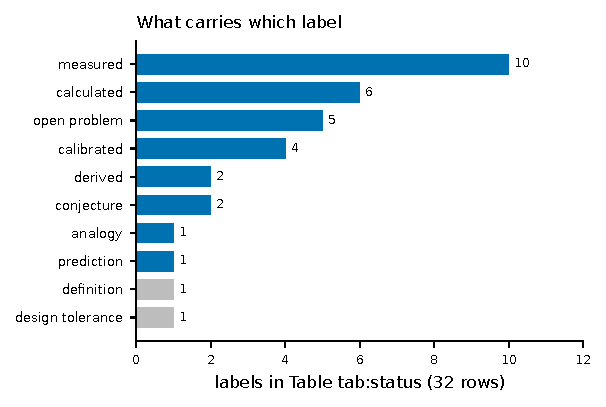
\includegraphics[width=0.62\textwidth]{figures/part6/fig_p4_24_labels.pdf}
\caption{Status labels in Table~\ref{tab:status}, counted from the table (32 rows; 10 carry MEASURED). Gray: rows whose status is a word
rather than a label. \observed}
\label{fig:p4_labels}
\end{figure}
\begin{figure}[htbp]\centering
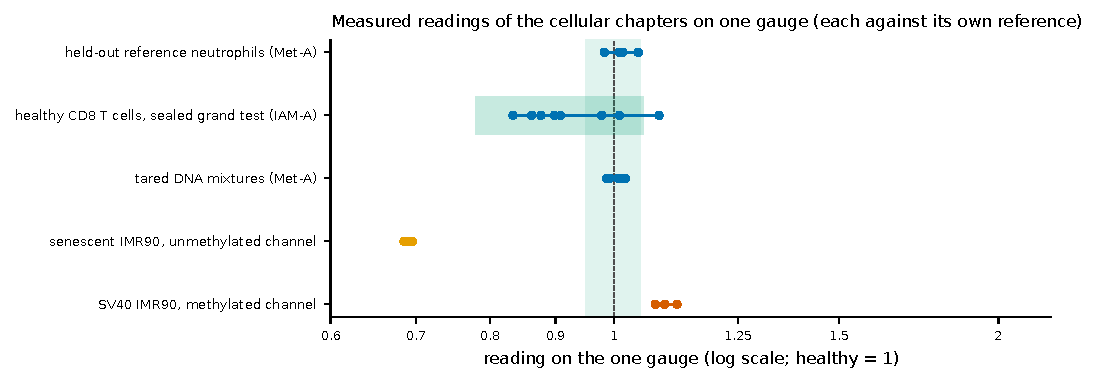
\includegraphics[width=0.98\textwidth]{figures/part6/fig_p4_24_summary.pdf}
\caption{Measured readings of Part~\ref{part:4} on the one gauge, each against its own healthy reference: held-out reference neutrophils
(Chapter~\ref{ch:meta}); healthy CD8 T cells of IAM-A's sealed grand test, each against its own loose share, with IAM-A's own Normal band (band v1, 0.779--1.055) shaded on its row (Chapter~\ref{ch:iama}); tared mixtures
(Chapter~\ref{ch:instrument}); IMR90 channels (Chapter~\ref{ch:gauge}). Normal shaded; log scale. \measured}
\label{fig:p4_summary}
\end{figure}
